% =================================================================
%  Savings accounts -- worked examples to go with the two worksheets
%  Change aspectratio=169 to 43 if your projector is 4:3.
%
%  Structure:
%    * the worked examples build up a step at a time: the table fills
%      row by row and the graph grows point by point alongside it, and
%      the formula card comes last;
%    * every mini-whiteboard question is a question slide with blanks,
%      followed by its own solution slide.
%
%  Everything that is not yet due is hidden rather than left out, so
%  the tables, the axes and the cards never move as a slide builds.
% =================================================================
\documentclass[aspectratio=169,12pt]{beamer}

\usetheme{default}
\setbeamertemplate{navigation symbols}{}

\usepackage[T1]{fontenc}
% lining, tabular figures: digits sit on the baseline and money columns line up
\usepackage[sfdefault,scaled=0.92,lining,tabular]{FiraSans}
\usepackage{tikz}
\usetikzlibrary{overlay-beamer-styles}
\usepackage{pgfplots}
\pgfplotsset{compat=1.18}
\usepackage{booktabs}
\usepackage{array}
\usepackage{colortbl}
\usepackage{tcolorbox}
\tcbuselibrary{skins}
% Maths is set in the text font, so the formulas and the prose match.
\usepackage[italic]{mathastext}

% ---------------- bank colours (match the worksheets) -------------
\definecolor{metroline}{HTML}{1F4E9C}
\definecolor{virgo}{HTML}{C62828}
\definecolor{coventree}{HTML}{2E7D32}
\definecolor{starlight}{HTML}{6A1B9A}
\definecolor{chace}{HTML}{00796B}
\definecolor{tesbury}{HTML}{E65100}
\definecolor{santandra}{HTML}{C62828}
\definecolor{nationworth}{HTML}{AD1457}
\definecolor{halifield}{HTML}{00796B}
\definecolor{answer}{HTML}{B3005E}

% ---------------- neutral palette ---------------------------------
\definecolor{slidehead}{HTML}{1C2B3A}   % titles and headings
\definecolor{ink}{HTML}{212B36}         % body text
\definecolor{inkmuted}{HTML}{6B7A8A}    % labels, axes, captions
\definecolor{hairline}{HTML}{DCE3EA}    % rules and card edges

\setbeamercolor{normal text}{fg=ink}
\setbeamercolor{structure}{fg=slidehead}
\setbeamertemplate{itemize items}[circle]
\arrayrulecolor{hairline}
\setlength{\heavyrulewidth}{0.5pt}
\setlength{\lightrulewidth}{0.4pt}
\renewcommand{\arraystretch}{1.05}

% A quiet frame number in the bottom corner. This counts frames rather
% than slides, so it does not move while a slide is building up.
\setbeamertemplate{footline}{%
  \hfill\textcolor{inkmuted}{\scriptsize\insertframenumber}\hspace*{4mm}%
  \vspace*{1.5mm}}

% ---------------- frame title -------------------------------------
\setbeamercolor{frametitle}{fg=white,bg=slidehead}
\setbeamertemplate{frametitle}{%
  \vskip1mm%
  \begin{tcolorbox}[enhanced,nobeforeafter,width=\linewidth,
      colback=slidehead,colframe=slidehead,arc=3mm,boxrule=0pt,
      left=3.5mm,right=3.5mm,top=1.2mm,bottom=1.2mm]
    \color{white}\large\bfseries\insertframetitle
  \end{tcolorbox}%
  \vskip1mm%
}

% ---------------- rounded cards -----------------------------------
% Flat fill, no outline, and a coloured edge down the left-hand side.
% A card for a table or a piece of explanation.
\newtcolorbox{card}[1][slidehead]{enhanced,nobeforeafter,box align=top,
  colback=#1!6,colframe=#1!6,boxrule=0pt,arc=2.5mm,
  borderline west={2.2pt}{0pt}{#1!75},
  left=3mm,right=3mm,top=1.5mm,bottom=1.5mm,
  halign upper=flush left,
  before upper={\def\cardaccent{#1}}}

% A card for a graph, so the plot sits on white.
\newtcolorbox{plotcard}[1][slidehead]{enhanced,nobeforeafter,box align=top,
  colback=white,colframe=hairline,boxrule=0.5pt,arc=2.5mm,
  left=1mm,right=1mm,top=1mm,bottom=0.5mm}

% A card for the calculation done straight from the formula.
\newtcolorbox{formulacard}[1][slidehead]{enhanced,nobeforeafter,box align=top,
  colback=white,colframe=hairline,boxrule=0.5pt,arc=2.5mm,
  borderline west={2.2pt}{0pt}{#1!75},
  left=3mm,right=3mm,top=1.2mm,bottom=1.2mm,
  fontupper=\footnotesize, halign upper=flush left,
  before upper={\def\cardaccent{#1}}}

% The heading on a card, in the colour of that account.
\newcommand{\cardhead}[1]{{\color{\cardaccent}\bfseries #1}}

% ---------------- answers -----------------------------------------
% \ablank draws an empty answer box on a question slide and \ashow
% prints the answer on the solution slide that follows it. Both take
% the answer as their argument, so the question text can be written
% once and used on both slides.
\newcommand{\ablank}[1]{%
  \tikz[baseline=-0.7ex]{%
    \node[draw=hairline,line width=0.8pt,fill=slidehead!4,
          rounded corners=2pt,minimum width=24mm,minimum height=6mm,
          inner sep=0pt] {};}}
\newcommand{\ashow}[1]{\textcolor{answer}{\textbf{#1}}}

% \pounds usable inside maths
\newcommand{\pnd}{\mbox{\pounds}}

% ---------------- mini-whiteboard and solution banners ------------
\newcommand{\wb}{%
  \tcbox[on line,boxsep=0.8pt,left=4pt,right=4pt,top=1.2pt,bottom=1.2pt,
         colback=white,colframe=white,arc=3.5pt,boxrule=0pt]
        {\color{slidehead}\scriptsize\bfseries MINI-WHITEBOARDS}}

\newcommand{\sol}{%
  \tcbox[on line,boxsep=0.8pt,left=4pt,right=4pt,top=1.2pt,bottom=1.2pt,
         colback=answer,colframe=answer,arc=3.5pt,boxrule=0pt]
        {\color{white}\scriptsize\bfseries SOLUTION}}

% The gap between questions. A question slide has nothing else on it, so
% it can afford to be roomy; the solution slide also carries the working.
\newlength{\qgap}
\setlength{\qgap}{2.5mm}

% The centred block a question slide is set in.
\newenvironment{questionblock}
  {\vspace{2mm}\begin{center}\begin{minipage}{0.72\textwidth}%
   \large\setlength{\qgap}{4mm}}
  {\end{minipage}\end{center}}

% ---------------- a bank name badge ------------------------------
\newcommand{\bank}[2]{%
  \tcbox[on line,boxsep=1pt,left=5pt,right=5pt,top=1.8pt,bottom=1.8pt,
         colback=#1,colframe=#1,arc=4.5pt,boxrule=0pt]
        {\color{white}\small\bfseries #2}}

% ---------------- shared plot style ------------------------------
% Thin grey axes with no arrow tips, faint grid, and a legend that
% floats on the plot rather than sitting in a box.
\pgfplotsset{
  moneyaxis/.style={
    width=6.4cm, height=4.0cm,
    xlabel={years}, ylabel={amount (\pounds)},
    xlabel style={font=\scriptsize,color=inkmuted},
    ylabel style={font=\scriptsize,color=inkmuted},
    tick label style={font=\scriptsize,color=inkmuted},
    grid=major, grid style={hairline,line width=0.4pt},
    axis lines=left,
    axis line style={draw=hairline,line width=0.6pt,-},
    tick style={draw=hairline},
    enlarge x limits=0.06,
    scaled y ticks=false,
    y tick label style={/pgf/number format/fixed,
                        /pgf/number format/1000 sep={}},
    legend style={font=\scriptsize,draw=none,fill=white,
                  fill opacity=0.85,text opacity=1,
                  at={(0.02,0.99)},anchor=north west,
                  inner sep=1.5pt,nodes={inner sep=1.5pt}},
    legend cell align=left,
  }
}

% ---------------- building a table up row by row ------------------
% Each cell is uncovered from overlay #1 onwards. The whole table is
% typeset from the start, so the column widths and the rows below it
% do not move as the rows appear.
\newcommand{\rowtwo}[3]{\uncover<#1->{#2} & \uncover<#1->{#3}\\}
\newcommand{\rowthree}[4]{%
  \uncover<#1->{#2} & \uncover<#1->{#3} & \uncover<#1->{#4}\\}

% ---------------- building a graph up point by point --------------
% \pt draws a single point, \seg one straight segment from #3 to #4,
% and \curveseg the piece of a curve between x = #3 and x = #4. Each
% is hidden until overlay #1 rather than left out, so the axis keeps
% its size and the earlier parts of the line stay put.
%   #1 first overlay   #2 plot style   #3, #4 coordinates
\newcommand{\pt}[3]{%
  \addplot[#2,visible on=<#1->,forget plot] coordinates {#3};}
\newcommand{\seg}[4]{%
  \addplot[#2,visible on=<#1->,forget plot] coordinates {#3#4};}
%   #1 first overlay  #2 style  #3 from  #4 to  #5 expression in x
\newcommand{\curveseg}[5]{%
  \addplot[#2,visible on=<#1->,forget plot,domain=#3:#4,samples=41] {#5};}

% Legends are built from \addlegendimage so that they are complete from
% the first overlay, while the plots themselves are all "forget plot".
\newcommand{\legendfor}[2]{\addlegendimage{#1}\addlegendentry{#2}}

% A rounded label marking the years a saver cannot withdraw the money.
%   #1 colour   #2 x position   #3 y position
\newcommand{\lockedlabel}[3]{%
  \node[fill=#1!12,rounded corners=3pt,inner xsep=4pt,inner ysep=2.5pt,
        font=\tiny,text=#1,align=center] at (axis cs:#2,#3) {locked in};}

\title{Savings accounts: which is the best deal?}
\subtitle{Worked solutions}
\date{}

\begin{document}

\begin{frame}[plain]
  \vfill
  \hspace*{6mm}%
  \begin{minipage}{0.86\textwidth}
    {\color{inkmuted}\small\bfseries WORKED SOLUTIONS}\\[3mm]
    {\color{slidehead}\fontsize{24}{28}\selectfont\bfseries
     Savings accounts:\\which is the best deal?}\\[4mm]
    \textcolor{slidehead!75}{\rule{28mm}{2.2pt}}\\[4mm]
    {\color{inkmuted}\small All bank names and interest rates are made up.}
  \end{minipage}
  \vfill
\end{frame}

% =================================================================
% The two tables fill in step by step side by side, so the same year
% can be compared in both accounts before the next one appears.
\begin{frame}{Two ways of paying interest}
\begin{columns}[T,onlytextwidth]
\begin{column}{0.48\textwidth}
  \begin{card}[coventree]
    \textbf{Simple interest}\\[1mm]
    \footnotesize
    Interest is worked out on the amount you first paid in, every year.
    \vspace{1.5mm}

    \pounds200 at 10\% simple interest:\\[1mm]
    \begin{tabular}{@{}lll@{}}
      \rowthree{2}{Year 1}{\pounds20}{\pounds220}
      \rowthree{3}{Year 2}{\pounds20}{\pounds240}
      \rowthree{4}{Year 3}{\pounds20}{\pounds260}
    \end{tabular}\\[1.5mm]
    \uncover<5->{The interest is \pounds20 every year.}
  \end{card}
\end{column}
\begin{column}{0.48\textwidth}
  \begin{card}[starlight]
    \textbf{Compound interest}\\[1mm]
    \footnotesize
    Interest is worked out on the amount in the account, so we earn
    interest on our interest.
    \vspace{1.5mm}

    \pounds200 at 10\% compound interest:\\[1mm]
    \begin{tabular}{@{}lll@{}}
      \rowthree{2}{Year 1}{\pounds20.00}{\pounds220.00}
      \rowthree{3}{Year 2}{\pounds22.00}{\pounds242.00}
      \rowthree{4}{Year 3}{\pounds24.20}{\pounds266.20}
    \end{tabular}\\[1.5mm]
    \uncover<5->{The interest grows each year.}
  \end{card}
\end{column}
\end{columns}

\vspace{2mm}
\uncover<5->{%
\begin{formulacard}[slidehead]
  \cardhead{The two formulas.}
  $P$ is the amount paid in, $r$ is the interest rate written as a decimal
  and $n$ is the number of years.\\[1mm]
  \centering
  simple interest: total $= P(1+rn)$
  \qquad\qquad
  compound interest: total $= P(1+r)^{n}$
\end{formulacard}}
\end{frame}

% =================================================================
\begin{frame}{\bank{coventree}{Coventree} Standard Saver: 5\% simple interest}
\textbf{Fay puts in \pounds250 and leaves it for 3 years.}
\vspace{0.6mm}

\begin{columns}[T,onlytextwidth]
\begin{column}{0.44\textwidth}
  \begin{card}[coventree]
    \footnotesize
    5\% of \pounds250 is \pounds12.50, and the account pays that
    \emph{every} year.\\[1.5mm]
    \begin{tabular}{@{}lrr@{}}
      \toprule
      & interest & total\\
      \midrule
      \rowthree{1}{Start}{}{\pounds250.00}
      \rowthree{2}{Year 1}{\pounds12.50}{\pounds262.50}
      \rowthree{3}{Year 2}{\pounds12.50}{\pounds275.00}
      \rowthree{4}{Year 3}{\pounds12.50}{\pounds287.50}
      \bottomrule
    \end{tabular}
  \end{card}

  \vspace{1.2mm}
  \uncover<5->{%
  \begin{formulacard}[coventree]
    \cardhead{Using the formula}\\[0.6mm]
    interest $= P \times r \times n$\\[0.4mm]
    \hspace*{3mm}$= \pnd 250 \times 0.05 \times 3 = \pnd 37.50$\\[0.4mm]
    total $= \pnd 250 + \pnd 37.50 = \pnd 287.50$
  \end{formulacard}}
\end{column}
\begin{column}{0.54\textwidth}
  \begin{plotcard}[coventree]
  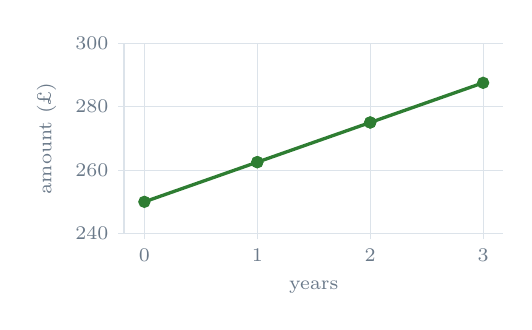
\begin{tikzpicture}
    \begin{axis}[moneyaxis, xmin=0,xmax=3,ymin=240,ymax=300,xtick={0,1,2,3}]
      \pt{1}{coventree,mark=*,mark size=1.6pt}{(0,250)}
      \seg{2}{coventree,very thick,mark=*,mark size=1.6pt}{(0,250)}{(1,262.5)}
      \seg{3}{coventree,very thick,mark=*,mark size=1.6pt}{(1,262.5)}{(2,275)}
      \seg{4}{coventree,very thick,mark=*,mark size=1.6pt}{(2,275)}{(3,287.5)}
    \end{axis}
  \end{tikzpicture}
  \end{plotcard}\\[1mm]
  \uncover<5->{\footnotesize Simple interest gives a \textbf{straight line}.}
\end{column}
\end{columns}
\end{frame}

% =================================================================
% Amara: question slide, then solution slide. The questions themselves
% live in one macro so the two slides cannot drift apart; #1 is
% \ablank on the question slide and \ashow on the solution slide.
\newcommand{\amaraQuestions}[1]{%
  How much interest each year? \hfill #1{\pounds12}\\[\qgap]
  How much interest altogether? \hfill #1{\pounds48}\\[\qgap]
  Total at the end? \hfill #1{\pounds168}}

\begin{frame}{\wb\ \ \bank{metroline}{Metroline Bank} 10\% simple interest}
\begin{questionblock}
  \textbf{Amara puts in \pounds120 and leaves it for 4 years.}\\[7mm]
  \amaraQuestions{\ablank}
\end{questionblock}
\end{frame}

\begin{frame}{\sol\ \ \bank{metroline}{Metroline Bank} 10\% simple interest}
\textbf{Amara puts in \pounds120 and leaves it for 4 years.}
\vspace{2mm}

\begin{columns}[T,onlytextwidth]
\begin{column}{0.5\textwidth}
  \amaraQuestions{\ashow}

  \vspace{4mm}
  \uncover<6->{%
  \begin{formulacard}[metroline]
    \cardhead{Using the formula}\\[0.6mm]
    interest $= P \times r \times n$\\[0.4mm]
    \hspace*{3mm}$= \pnd 120 \times 0.10 \times 4 = \pnd 48$\\[0.4mm]
    total $= \pnd 120 + \pnd 48 = \pnd 168$
  \end{formulacard}}
\end{column}
\begin{column}{0.46\textwidth}
  \begin{card}[metroline]
    \footnotesize
    \begin{tabular}{@{}lrr@{}}
      \toprule
      & interest & total\\
      \midrule
      \rowthree{1}{Start}{}{\pounds120}
      \rowthree{2}{Year 1}{\pounds12}{\pounds132}
      \rowthree{3}{Year 2}{\pounds12}{\pounds144}
      \rowthree{4}{Year 3}{\pounds12}{\pounds156}
      \rowthree{5}{Year 4}{\pounds12}{\pounds168}
      \bottomrule
    \end{tabular}
  \end{card}
\end{column}
\end{columns}
\end{frame}

% =================================================================
\begin{frame}{\bank{starlight}{Starlight Bank} Steady Saver: 5\% compound interest}
\textbf{Fay puts in \pounds250 and leaves it for 3 years.}
\vspace{1mm}

\begin{columns}[T,onlytextwidth]
\begin{column}{0.44\textwidth}
  \begin{card}[starlight]
    \footnotesize
    We multiply by $1.05$ each year.\\[1.5mm]
    \begin{tabular}{@{}lrr@{}}
      \toprule
      & interest & total\\
      \midrule
      \rowthree{1}{Start}{}{\pounds250.00}
      \rowthree{2}{Year 1}{\pounds12.50}{\pounds262.50}
      \rowthree{3}{Year 2}{\pounds13.13}{\pounds275.63}
      \rowthree{4}{Year 3}{\pounds13.78}{\pounds289.41}
      \bottomrule
    \end{tabular}
  \end{card}

  \vspace{0.8mm}
  \uncover<5->{%
  \begin{formulacard}[starlight]
    \cardhead{Using the formula}\\[0.6mm]
    total $= P(1+r)^{n}$\\[0.4mm]
    \hspace*{3mm}$= \pnd 250 \times 1.05^{3} = \pnd 289.41$\\[0.4mm]
    interest $= \pnd 289.41 - \pnd 250 = \pnd 39.41$
  \end{formulacard}}
\end{column}
\begin{column}{0.54\textwidth}
  \begin{plotcard}[starlight]
  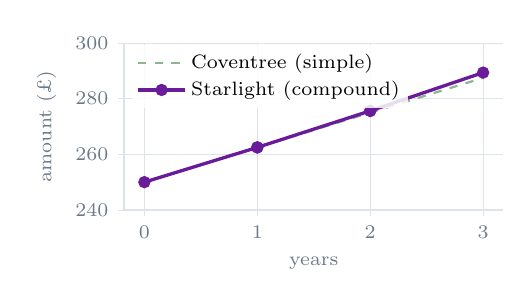
\begin{tikzpicture}
    \begin{axis}[moneyaxis, height=3.7cm,
                 xmin=0,xmax=3,ymin=240,ymax=300,xtick={0,1,2,3}]
      \legendfor{coventree!55,thick,dashed}{Coventree (simple)}
      \legendfor{starlight,very thick,mark=*,mark size=1.6pt}{Starlight (compound)}
      \seg{2}{coventree!55,thick,dashed}{(0,250)}{(1,262.5)}
      \seg{3}{coventree!55,thick,dashed}{(1,262.5)}{(2,275)}
      \seg{4}{coventree!55,thick,dashed}{(2,275)}{(3,287.5)}
      \pt{1}{starlight,mark=*,mark size=1.6pt}{(0,250)}
      \seg{2}{starlight,very thick,mark=*,mark size=1.6pt}{(0,250)}{(1,262.5)}
      \seg{3}{starlight,very thick,mark=*,mark size=1.6pt}{(1,262.5)}{(2,275.63)}
      \seg{4}{starlight,very thick,mark=*,mark size=1.6pt}{(2,275.63)}{(3,289.41)}
    \end{axis}
  \end{tikzpicture}
  \end{plotcard}\\[1mm]
  \uncover<5->{\footnotesize Same rate, same start --- but the line
  \textbf{bends upwards}.}
\end{column}
\end{columns}
\end{frame}

% =================================================================
% Ben: question slide, then solution slide.
\newcommand{\benQuestions}[1]{%
  What do we multiply by each year? \hfill #1{1.04}\\[\qgap]
  How much after 1 year? \hfill #1{\pounds208}\\[\qgap]
  How much after 2 years? \hfill #1{\pounds216.32}}

\begin{frame}{\wb\ \ \bank{chace}{Chace} 4\% compound interest}
\begin{questionblock}
  \textbf{Ben puts in \pounds200 and leaves it for 2 years.}\\[7mm]
  \benQuestions{\ablank}
\end{questionblock}
\end{frame}

\begin{frame}{\sol\ \ \bank{chace}{Chace} 4\% compound interest}
\textbf{Ben puts in \pounds200 and leaves it for 2 years.}
\vspace{2mm}

\begin{columns}[T,onlytextwidth]
\begin{column}{0.54\textwidth}
  \benQuestions{\ashow}

  \vspace{4mm}
  \uncover<4->{%
  \begin{formulacard}[chace]
    \cardhead{Using the formula}\\[0.6mm]
    total $= P(1+r)^{n}$\\[0.4mm]
    \hspace*{3mm}$= \pnd 200 \times 1.04^{2} = \pnd 216.32$\\[0.4mm]
    The second year's interest is \pounds8.32 rather than \pounds8
    because it is 4\% of \pounds208, not 4\% of \pounds200.
  \end{formulacard}}
\end{column}
\begin{column}{0.42\textwidth}
  \begin{card}[chace]
    \footnotesize
    \begin{tabular}{@{}lrr@{}}
      \toprule
      & interest & total\\
      \midrule
      \rowthree{1}{Start}{}{\pounds200.00}
      \rowthree{2}{Year 1}{\pounds8.00}{\pounds208.00}
      \rowthree{3}{Year 2}{\pounds8.32}{\pounds216.32}
      \bottomrule
    \end{tabular}
  \end{card}
\end{column}
\end{columns}
\end{frame}

% =================================================================
\begin{frame}{Five years: the gap opens up}
\begin{columns}[T,onlytextwidth]
\begin{column}{0.48\textwidth}
  \begin{card}
    \footnotesize
    \pounds250 in each account, both paying 5\%.\\[1.5mm]
    \begin{tabular}{@{}lrr@{}}
      \toprule
      & Coventree & Starlight\\
      & simple & compound\\
      \midrule
      \rowthree{1}{Year 1}{\pounds262.50}{\pounds262.50}
      \rowthree{2}{Year 2}{\pounds275.00}{\pounds275.63}
      \rowthree{3}{Year 3}{\pounds287.50}{\pounds289.41}
      \rowthree{4}{Year 4}{\pounds300.00}{\pounds303.88}
      \rowthree{5}{Year 5}{\pounds312.50}{\pounds319.07}
      \bottomrule
    \end{tabular}
  \end{card}

  \vspace{1.2mm}
  \uncover<6->{%
  \begin{formulacard}
    \cardhead{After 5 years}\\[0.6mm]
    simple: $\pnd 250 (1 + 0.05 \times 5) = \pnd 312.50$\\[0.4mm]
    compound: $\pnd 250 \times 1.05^{5} = \pnd 319.07$
  \end{formulacard}}
\end{column}
\begin{column}{0.5\textwidth}
  \begin{plotcard}
  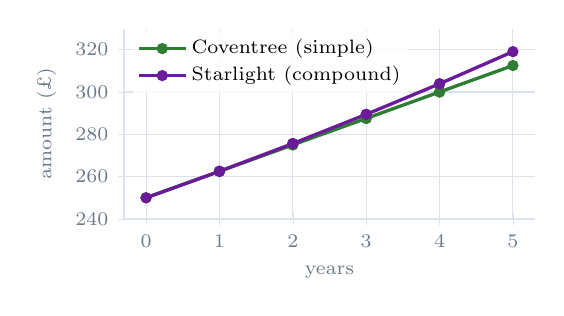
\begin{tikzpicture}
    \begin{axis}[moneyaxis, width=6.8cm, xmin=0,xmax=5,ymin=240,ymax=330,xtick={0,...,5}]
      \legendfor{coventree,very thick,mark=*,mark size=1.4pt}{Coventree (simple)}
      \legendfor{starlight,very thick,mark=*,mark size=1.4pt}{Starlight (compound)}
      \pt{1}{coventree,mark=*,mark size=1.4pt}{(0,250)}
      \seg{1}{coventree,very thick,mark=*,mark size=1.4pt}{(0,250)}{(1,262.5)}
      \seg{2}{coventree,very thick,mark=*,mark size=1.4pt}{(1,262.5)}{(2,275)}
      \seg{3}{coventree,very thick,mark=*,mark size=1.4pt}{(2,275)}{(3,287.5)}
      \seg{4}{coventree,very thick,mark=*,mark size=1.4pt}{(3,287.5)}{(4,300)}
      \seg{5}{coventree,very thick,mark=*,mark size=1.4pt}{(4,300)}{(5,312.5)}
      \seg{1}{starlight,very thick,mark=*,mark size=1.4pt}{(0,250)}{(1,262.5)}
      \seg{2}{starlight,very thick,mark=*,mark size=1.4pt}{(1,262.5)}{(2,275.63)}
      \seg{3}{starlight,very thick,mark=*,mark size=1.4pt}{(2,275.63)}{(3,289.41)}
      \seg{4}{starlight,very thick,mark=*,mark size=1.4pt}{(3,289.41)}{(4,303.88)}
      \seg{5}{starlight,very thick,mark=*,mark size=1.4pt}{(4,303.88)}{(5,319.07)}
    \end{axis}
  \end{tikzpicture}
  \end{plotcard}\\[1mm]
  \uncover<6->{\footnotesize The gap gets wider every year.}
\end{column}
\end{columns}
\end{frame}

% =================================================================
\begin{frame}{Twenty-five years of the same 5\%}
\begin{columns}[T,onlytextwidth]
\begin{column}{0.46\textwidth}
  \begin{card}
    \footnotesize
    \pounds250 in each account, still at 5\%.\\[1.5mm]
    \begin{tabular}{@{}lrr@{}}
      \toprule
      & Coventree & Starlight\\
      & simple & compound\\
      \midrule
      \rowthree{1}{Year 5}{\pounds312.50}{\pounds319.07}
      \rowthree{2}{Year 10}{\pounds375.00}{\pounds407.22}
      \rowthree{3}{Year 15}{\pounds437.50}{\pounds519.73}
      \rowthree{4}{Year 20}{\pounds500.00}{\pounds663.32}
      \rowthree{5}{Year 25}{\pounds562.50}{\pounds846.59}
      \bottomrule
    \end{tabular}
  \end{card}

  \vspace{1.2mm}
  \uncover<6->{%
  \begin{formulacard}
    \cardhead{After 25 years}\\[0.6mm]
    simple: $\pnd 250 (1 + 0.05 \times 25) = \pnd 562.50$\\[0.4mm]
    compound: $\pnd 250 \times 1.05^{25} = \pnd 846.59$
  \end{formulacard}}
\end{column}
\begin{column}{0.52\textwidth}
  \begin{plotcard}
  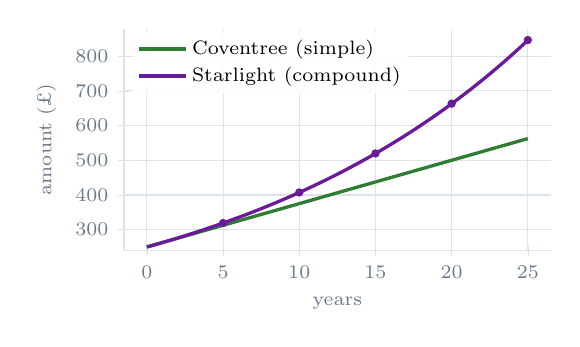
\begin{tikzpicture}
    \begin{axis}[moneyaxis, width=7cm, height=4.4cm,
                 xmin=0,xmax=25,ymin=240,ymax=880,
                 xtick={0,5,10,15,20,25}, ytick={300,400,500,600,700,800}]
      \legendfor{coventree,very thick}{Coventree (simple)}
      \legendfor{starlight,very thick}{Starlight (compound)}
      \curveseg{1}{coventree,very thick}{0}{5}{250*(1+0.05*x)}
      \curveseg{2}{coventree,very thick}{5}{10}{250*(1+0.05*x)}
      \curveseg{3}{coventree,very thick}{10}{15}{250*(1+0.05*x)}
      \curveseg{4}{coventree,very thick}{15}{20}{250*(1+0.05*x)}
      \curveseg{5}{coventree,very thick}{20}{25}{250*(1+0.05*x)}
      \curveseg{1}{starlight,very thick}{0}{5}{250*exp(x*ln(1.05))}
      \curveseg{2}{starlight,very thick}{5}{10}{250*exp(x*ln(1.05))}
      \curveseg{3}{starlight,very thick}{10}{15}{250*exp(x*ln(1.05))}
      \curveseg{4}{starlight,very thick}{15}{20}{250*exp(x*ln(1.05))}
      \curveseg{5}{starlight,very thick}{20}{25}{250*exp(x*ln(1.05))}
      \pt{1}{starlight,mark=*,mark size=1.3pt}{(5,319.07)}
      \pt{2}{starlight,mark=*,mark size=1.3pt}{(10,407.22)}
      \pt{3}{starlight,mark=*,mark size=1.3pt}{(15,519.73)}
      \pt{4}{starlight,mark=*,mark size=1.3pt}{(20,663.32)}
      \pt{5}{starlight,mark=*,mark size=1.3pt}{(25,846.59)}
    \end{axis}
  \end{tikzpicture}
  \end{plotcard}\\[1mm]
  \uncover<6->{\footnotesize The simple interest line keeps the same gradient,
  while the compound curve gets steeper every year. After 25 years the
  difference is \pounds284.09.}
\end{column}
\end{columns}
\end{frame}

% =================================================================
\begin{frame}{\bank{virgo}{Virgo Money} 8\% compound over thirty years}
\begin{columns}[T,onlytextwidth]
\begin{column}{0.48\textwidth}
  \begin{card}[virgo]
    \footnotesize
    Dev pays in \pounds1000 and leaves it alone. The second column is the
    same \pounds1000 at 8\% \emph{simple} interest.\\[1.5mm]
    \begin{tabular}{@{}lrr@{}}
      \toprule
      & simple & compound\\
      \midrule
      \rowthree{1}{Year 10}{\pounds1800}{\pounds2158.92}
      \rowthree{2}{Year 20}{\pounds2600}{\pounds4660.96}
      \rowthree{3}{Year 30}{\pounds3400}{\pounds10062.66}
      \bottomrule
    \end{tabular}
  \end{card}

  \vspace{1.2mm}
  \uncover<4->{%
  \begin{formulacard}[virgo]
    \cardhead{After 30 years}\\[0.6mm]
    simple: $\pnd 1000 (1 + 0.08 \times 30) = \pnd 3400$\\[0.4mm]
    compound: $\pnd 1000 \times 1.08^{30} = \pnd 10062.66$
  \end{formulacard}}
\end{column}
\begin{column}{0.50\textwidth}
  \begin{plotcard}[virgo]
  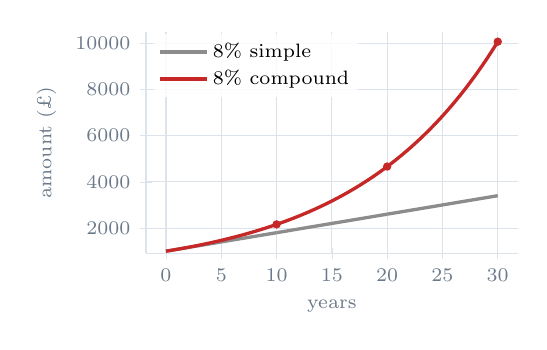
\begin{tikzpicture}
    \begin{axis}[moneyaxis, width=6.3cm, height=4.4cm,
                 xmin=0,xmax=30,ymin=900,ymax=10500,
                 xtick={0,5,10,15,20,25,30},
                 ytick={2000,4000,6000,8000,10000}]
      \legendfor{black!45,very thick}{8\% simple}
      \legendfor{virgo,very thick}{8\% compound}
      \curveseg{1}{black!45,very thick}{0}{10}{1000*(1+0.08*x)}
      \curveseg{2}{black!45,very thick}{10}{20}{1000*(1+0.08*x)}
      \curveseg{3}{black!45,very thick}{20}{30}{1000*(1+0.08*x)}
      \curveseg{1}{virgo,very thick}{0}{10}{1000*exp(x*ln(1.08))}
      \curveseg{2}{virgo,very thick}{10}{20}{1000*exp(x*ln(1.08))}
      \curveseg{3}{virgo,very thick}{20}{30}{1000*exp(x*ln(1.08))}
      \pt{1}{virgo,mark=*,mark size=1.3pt}{(10,2158.92)}
      \pt{2}{virgo,mark=*,mark size=1.3pt}{(20,4660.96)}
      \pt{3}{virgo,mark=*,mark size=1.3pt}{(30,10062.66)}
    \end{axis}
  \end{tikzpicture}
  \end{plotcard}\\[1mm]
  \uncover<4->{\footnotesize The compound total doubles roughly every 9 years:
  about \pounds2000 at 9 years, \pounds4000 at 18 years and \pounds8000 at
  27 years.}
\end{column}
\end{columns}
\end{frame}

% =================================================================
% Priya: question slide, then solution slide.
\newcommand{\priyaQuestions}[1]{%
  What do we multiply by each year? \hfill #1{1.06}\\[\qgap]
  How much after 10 years? \hfill #1{\pounds895.42}\\[\qgap]
  After how many whole years is there more than \pounds1000?
  \hfill #1{12 years}}

\begin{frame}{\wb\ \ How long does the money take to double?}
\begin{questionblock}
  {\normalsize\raggedright\bank{starlight}{Starlight Bank} also offers 6\%
   compound interest per year.\par}
  \vspace{3mm}

  \textbf{Priya pays in \pounds500 and leaves it there.}\\[7mm]
  \priyaQuestions{\ablank}
\end{questionblock}
\end{frame}

\begin{frame}{\sol\ \ How long does the money take to double?}
\bank{starlight}{Starlight Bank} 6\% compound interest per year.
\textbf{Priya pays in \pounds500.}
\vspace{2mm}

\begin{columns}[T,onlytextwidth]
\begin{column}{0.52\textwidth}
  \priyaQuestions{\ashow}

  \vspace{3mm}
  \uncover<4->{%
  {\footnotesize At 6\% \emph{simple} interest the same \pounds500 does not
  pass \pounds1000 until year 17, because
  $\pnd 500 (1 + 0.06 \times 17) = \pnd 1010$.}}
\end{column}
\begin{column}{0.44\textwidth}
  \begin{card}[starlight]
    \footnotesize
    \begin{tabular}{@{}lr@{}}
      \toprule
      & total\\
      \midrule
      \rowtwo{1}{Year 10}{\pounds895.42}
      \rowtwo{2}{Year 11}{\pounds949.15}
      \rowtwo{3}{Year 12}{\pounds1006.10}
      \bottomrule
    \end{tabular}
  \end{card}

  \vspace{1.2mm}
  \uncover<4->{%
  \begin{formulacard}[starlight]
    $\pnd 500 \times 1.06^{12} = \pnd 1006.10$\\[0.6mm]
    \ashow{Compound interest doubles the money in 12 years, simple
    interest in 17.}
  \end{formulacard}}
\end{column}
\end{columns}
\end{frame}

% =================================================================
\begin{frame}{\bank{tesbury}{Tesbury Bank} 6\% simple --- but locked in for 2 years}
\textbf{Chloe puts in \pounds400 and leaves it for 4 years.}
\vspace{1.5mm}

\begin{columns}[T,onlytextwidth]
\begin{column}{0.42\textwidth}
  \begin{card}[tesbury]
    \footnotesize
    6\% of \pounds400 is \pounds24 every year.\\[1.5mm]
    \begin{tabular}{@{}lrr@{}}
      \toprule
      & interest & total\\
      \midrule
      \rowthree{1}{Start}{}{\pounds400}
      \rowthree{2}{Year 1}{\pounds24}{\pounds424}
      \rowthree{3}{Year 2}{\pounds24}{\pounds448}
      \rowthree{4}{Year 3}{\pounds24}{\pounds472}
      \rowthree{5}{Year 4}{\pounds24}{\pounds496}
      \bottomrule
    \end{tabular}
  \end{card}

  \vspace{1.2mm}
  \uncover<6->{%
  \begin{formulacard}[tesbury]
    \cardhead{Using the formula}\\[0.6mm]
    total $= P(1+rn)$\\[0.4mm]
    \hspace*{3mm}$= \pnd 400 (1 + 0.06 \times 4) = \pnd 496$
  \end{formulacard}}
\end{column}
\begin{column}{0.56\textwidth}
  \begin{plotcard}[tesbury]
  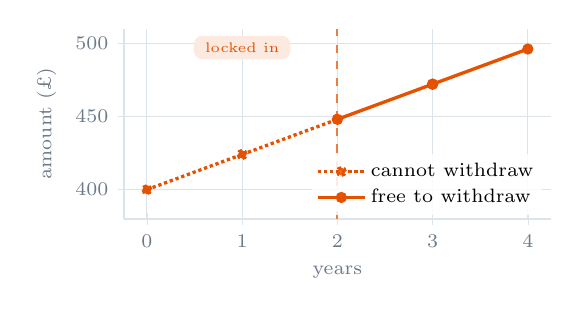
\begin{tikzpicture}
    \begin{axis}[moneyaxis, width=7cm, xmin=0,xmax=4,ymin=380,ymax=510,xtick={0,...,4},
                 legend style={at={(0.98,0.02)},anchor=south east}]
      \draw[tesbury!75,dashed,thick] (axis cs:2,380) -- (axis cs:2,510);
      \lockedlabel{tesbury}{1}{497}
      \legendfor{tesbury,very thick,densely dotted,mark=*,mark size=1.4pt}
                {cannot withdraw}
      \legendfor{tesbury,very thick,mark=*,mark size=1.4pt}{free to withdraw}
      \pt{1}{tesbury,mark=*,mark size=1.4pt}{(0,400)}
      \seg{2}{tesbury,very thick,densely dotted,mark=*,mark size=1.4pt}{(0,400)}{(1,424)}
      \seg{3}{tesbury,very thick,densely dotted,mark=*,mark size=1.4pt}{(1,424)}{(2,448)}
      \seg{4}{tesbury,very thick,mark=*,mark size=1.4pt}{(2,448)}{(3,472)}
      \seg{5}{tesbury,very thick,mark=*,mark size=1.4pt}{(3,472)}{(4,496)}
    \end{axis}
  \end{tikzpicture}
  \end{plotcard}\\[1mm]
  \uncover<6->{\footnotesize The \textbf{dotted} part is while the money is
  locked in.}
\end{column}
\end{columns}
\end{frame}

% =================================================================
% Erin: question slide, then solution slide.
\newcommand{\erinOffers}{%
  \bank{virgo}{Virgo Money} 8\% \textbf{compound} per year\\[4mm]
  \bank{tesbury}{Tesbury Bank} 6\% \textbf{simple} per year}

\begin{frame}{\wb\ \ Which account, and by how much?}
\begin{questionblock}
  \textbf{Erin has \pounds600 to save for 2 years.}\\[7mm]
  \erinOffers\\[7mm]
  Which gives her more, and what is the difference?
\end{questionblock}
\end{frame}

\begin{frame}{\sol\ \ Which account, and by how much?}
\textbf{Erin has \pounds600 to save for 2 years.}
\vspace{2mm}

\begin{columns}[T,onlytextwidth]
\begin{column}{0.5\textwidth}
  \erinOffers\\[5mm]
  \uncover<3->{\ashow{Virgo pays her \pounds27.84 more.}}

  \vspace{3mm}
  \uncover<4->{%
  \begin{formulacard}
    \cardhead{Using the formulas}\\[0.6mm]
    Virgo: $\pnd 600 \times 1.08^{2} = \pnd 699.84$\\[0.4mm]
    Tesbury: $\pnd 600 (1 + 0.06 \times 2) = \pnd 672$
  \end{formulacard}}
\end{column}
\begin{column}{0.46\textwidth}
  \begin{card}
    \footnotesize
    \begin{tabular}{@{}lrr@{}}
      \toprule
      & Virgo & Tesbury\\
      \midrule
      \rowthree{1}{Start}{\pounds600.00}{\pounds600}
      \rowthree{2}{Year 1}{\pounds648.00}{\pounds636}
      \rowthree{3}{Year 2}{\pounds699.84}{\pounds672}
      \bottomrule
    \end{tabular}
  \end{card}
\end{column}
\end{columns}
\end{frame}

% =================================================================
\begin{frame}{\bank{santandra}{Santandra} 8\% compound --- locked in for 2 years}
\textbf{Dev puts in \pounds1000 and leaves it for 3 years.}
\vspace{1.5mm}

\begin{columns}[T,onlytextwidth]
\begin{column}{0.42\textwidth}
  \begin{card}[santandra]
    \footnotesize
    The multiplier is $1.08$, once for each year.\\[1.5mm]
    \begin{tabular}{@{}lrr@{}}
      \toprule
      & interest & total\\
      \midrule
      \rowthree{1}{Start}{}{\pounds1000.00}
      \rowthree{2}{Year 1}{\pounds80.00}{\pounds1080.00}
      \rowthree{3}{Year 2}{\pounds86.40}{\pounds1166.40}
      \rowthree{4}{Year 3}{\pounds93.31}{\pounds1259.71}
      \bottomrule
    \end{tabular}
  \end{card}

  \vspace{1.2mm}
  \uncover<5->{%
  \begin{formulacard}[santandra]
    \cardhead{Using the formula}\\[0.6mm]
    total $= P(1+r)^{n}$\\[0.4mm]
    \hspace*{3mm}$= \pnd 1000 \times 1.08^{3} = \pnd 1259.71$
  \end{formulacard}}
\end{column}
\begin{column}{0.56\textwidth}
  \begin{plotcard}[santandra]
  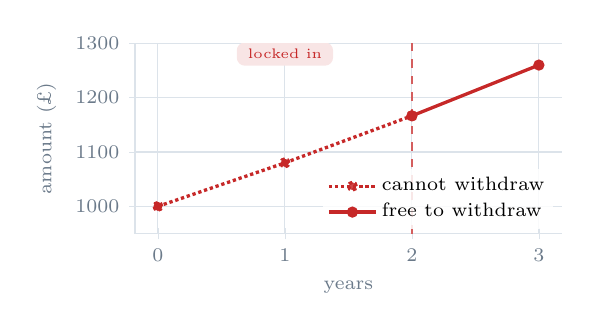
\begin{tikzpicture}
    \begin{axis}[moneyaxis, width=7cm, xmin=0,xmax=3,ymin=950,ymax=1300,xtick={0,1,2,3},
                 legend style={at={(0.98,0.02)},anchor=south east}]
      \draw[santandra!75,dashed,thick] (axis cs:2,950) -- (axis cs:2,1300);
      \lockedlabel{santandra}{1}{1280}
      \legendfor{santandra,very thick,densely dotted,mark=*,mark size=1.4pt}
                {cannot withdraw}
      \legendfor{santandra,very thick,mark=*,mark size=1.4pt}{free to withdraw}
      \pt{1}{santandra,mark=*,mark size=1.4pt}{(0,1000)}
      \seg{2}{santandra,very thick,densely dotted,mark=*,mark size=1.4pt}{(0,1000)}{(1,1080)}
      \seg{3}{santandra,very thick,densely dotted,mark=*,mark size=1.4pt}{(1,1080)}{(2,1166.4)}
      \seg{4}{santandra,very thick,mark=*,mark size=1.4pt}{(2,1166.4)}{(3,1259.71)}
    \end{axis}
  \end{tikzpicture}
  \end{plotcard}\\[1mm]
  \uncover<5->{\footnotesize Dev's money is locked in for the first 2 years,
  so this account is no use to him if he needs the cash sooner.}
\end{column}
\end{columns}
\end{frame}

% =================================================================
\begin{frame}{Read the small print}
\bank{metroline}{Metroline Bank} pays 10\%, the highest rate on the sheet,
but takes \pounds300 maximum. \textbf{Dev has \pounds1000 to save for 3 years.}
\vspace{1.5mm}

\begin{columns}[T,onlytextwidth]
\begin{column}{0.46\textwidth}
  \begin{card}[metroline]
    \footnotesize
    Only \pounds300 is allowed in the account.\\[1.5mm]
    \begin{tabular}{@{}lrr@{}}
      \toprule
      after 3 years & in account & total\\
      \midrule
      \rowthree{5}{Metroline}{\pounds390.00}{\pounds1090.00}
      \rowthree{5}{Virgo (8\%)}{\pounds1259.71}{\pounds1259.71}
      \bottomrule
    \end{tabular}
  \end{card}

  \vspace{1.2mm}
  \uncover<5->{%
  \begin{formulacard}[metroline]
    \cardhead{Using the formulas}\\[0.6mm]
    Metroline: $\pnd 300 (1 + 0.10 \times 3) = \pnd 390$,\\[0.4mm]
    \hspace*{3mm}and the \pounds700 left at home makes \pounds1090\\[0.4mm]
    Virgo: $\pnd 1000 \times 1.08^{3} = \pnd 1259.71$
  \end{formulacard}}
\end{column}
\begin{column}{0.52\textwidth}
  \begin{plotcard}[metroline]
  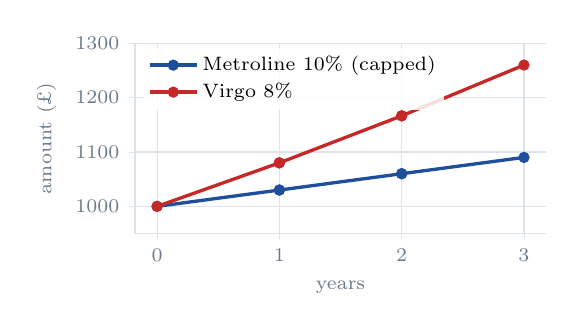
\begin{tikzpicture}
    \begin{axis}[moneyaxis, width=6.8cm, xmin=0,xmax=3,ymin=950,ymax=1300,xtick={0,1,2,3},
                 legend style={at={(0.02,0.98)}}]
      \legendfor{metroline,very thick,mark=*,mark size=1.4pt}{Metroline 10\% (capped)}
      \legendfor{virgo,very thick,mark=*,mark size=1.4pt}{Virgo 8\%}
      \pt{1}{metroline,mark=*,mark size=1.4pt}{(0,1000)}
      \seg{2}{metroline,very thick,mark=*,mark size=1.4pt}{(0,1000)}{(1,1030)}
      \seg{3}{metroline,very thick,mark=*,mark size=1.4pt}{(1,1030)}{(2,1060)}
      \seg{4}{metroline,very thick,mark=*,mark size=1.4pt}{(2,1060)}{(3,1090)}
      \seg{2}{virgo,very thick,mark=*,mark size=1.4pt}{(0,1000)}{(1,1080)}
      \seg{3}{virgo,very thick,mark=*,mark size=1.4pt}{(1,1080)}{(2,1166.4)}
      \seg{4}{virgo,very thick,mark=*,mark size=1.4pt}{(2,1166.4)}{(3,1259.71)}
    \end{axis}
  \end{tikzpicture}
  \end{plotcard}\\[1mm]
  \uncover<5->{\footnotesize The biggest percentage is not always the best deal.}
\end{column}
\end{columns}
\end{frame}

% =================================================================
% Aisha: question slide, then solution slide.
\newcommand{\aishaQuestions}[1]{%
  How much after 6 months? \hfill #1{\pounds510}\\[\qgap]
  How much after 12 months? \hfill #1{\pounds520.20}\\[\qgap]
  Is 2\% twice a year the same as 4\% once a year?}

\begin{frame}{\wb\ \ Interest paid twice a year}
\begin{questionblock}
  {\normalsize\raggedright\bank{halifield}{Halifield} Half-Year Saver: 2\%
   compound interest every six months.\par}
  \vspace{3mm}

  \textbf{Aisha puts in \pounds500 for one year.}\\[7mm]
  \aishaQuestions{\ablank}
\end{questionblock}
\end{frame}

\begin{frame}{\sol\ \ Interest paid twice a year}
\bank{halifield}{Halifield} Half-Year Saver: 2\% compound interest every six
months. \textbf{Aisha puts in \pounds500 for one year.}
\vspace{2mm}

\begin{columns}[T,onlytextwidth]
\begin{column}{0.5\textwidth}
  \aishaQuestions{\ashow}\\[1mm]
  \uncover<3->{\ashow{No --- \pounds520.20 against \pounds520.}}

  \vspace{1.6mm}
  \uncover<4->{%
  \begin{formulacard}[halifield]
    \cardhead{Using the formula}\\[0.6mm]
    Here $n = 2$, because the interest is added twice:\\[0.4mm]
    total $= \pnd 500 \times 1.02^{2} = \pnd 520.20$
  \end{formulacard}}
\end{column}
\begin{column}{0.46\textwidth}
  \begin{card}[halifield]
    \footnotesize
    \begin{tabular}{@{}lrr@{}}
      \toprule
      & interest & total\\
      \midrule
      \rowthree{1}{Start}{}{\pounds500.00}
      \rowthree{2}{6 months}{\pounds10.00}{\pounds510.00}
      \rowthree{3}{12 months}{\pounds10.20}{\pounds520.20}
      \bottomrule
    \end{tabular}\\[2mm]
    \uncover<4->{$1.02 \times 1.02 = 1.0404$, so it works out as 4.04\% for
    the year.}
  \end{card}
\end{column}
\end{columns}
\end{frame}

% =================================================================
% Sofia: question slide, then solution slide.
\newcommand{\sofiaQuestions}[1]{%
  How much interest in 2 years? \hfill #1{\pounds30}\\[\qgap]
  How much do the fees cost? \hfill #1{\pounds48}\\[\qgap]
  What is she left with? \hfill #1{\pounds232}}

\begin{frame}{\wb\ \ Challenge: a \pounds2 monthly fee}
\begin{questionblock}
  {\normalsize\raggedright\bank{nationworth}{Nationworth} Loyalty Saver: 6\%
   simple interest, \pounds2 fee every month.\par}
  \vspace{3mm}

  \textbf{Sofia puts in \pounds250 for 2 years.}\\[7mm]
  \sofiaQuestions{\ablank}
\end{questionblock}
\end{frame}

\begin{frame}{\sol\ \ Challenge: a \pounds2 monthly fee}
\bank{nationworth}{Nationworth} Loyalty Saver: 6\% simple interest, \pounds2
fee every month. \textbf{Sofia puts in \pounds250 for 2 years.}
\vspace{2mm}

\begin{columns}[T,onlytextwidth]
\begin{column}{0.5\textwidth}
  \sofiaQuestions{\ashow}

  \vspace{3.4mm}
  \uncover<5->{%
  \begin{formulacard}[nationworth]
    \cardhead{Using the formula}\\[0.6mm]
    interest $= P \times r \times n$\\[0.4mm]
    \hspace*{3mm}$= \pnd 250 \times 0.06 \times 2 = \pnd 30$\\[0.4mm]
    How much would she need to pay in before this account stops losing
    her money?
  \end{formulacard}}
\end{column}
\begin{column}{0.46\textwidth}
  \begin{card}[nationworth]
    \footnotesize
    \begin{tabular}{@{}lr@{}}
      \toprule
      \rowtwo{1}{Paid in}{\pounds250}
      \rowtwo{2}{Interest (2 years)}{$+$ \pounds30}
      \rowtwo{3}{Fees ($24 \times 2$)}{$-$ \pounds48}
      \midrule
      \rowtwo{4}{\textbf{Total}}{\textbf{\pounds232}}
      \bottomrule
    \end{tabular}\\[2mm]
    \uncover<4->{\ashow{She ends up with less than she started with.}}
  \end{card}
\end{column}
\end{columns}
\end{frame}

% =================================================================
\begin{frame}{Choosing an account}
\begin{columns}[T,onlytextwidth]
\begin{column}{0.56\textwidth}
  \begin{card}[slidehead]
    \small
    \begin{itemize}[<+->]\itemsep=1.4mm
      \item \textbf{Simple} interest is the same amount every year.
            \textbf{Compound} interest grows.
      \item At the same rate, compound interest always pays at least as
            much, and the gap grows the longer the money is left.
      \item A big percentage is no use if there is a \textbf{maximum} you
            can pay in.
      \item A \textbf{locked} account is no use if you need the money sooner.
      \item A \textbf{fee} can swallow the interest completely.
    \end{itemize}
  \end{card}
\end{column}
\begin{column}{0.42\textwidth}
  \begin{formulacard}[slidehead]
    \cardhead{The two formulas}\\[1.5mm]
    simple: total $= P(1+rn)$\\[1mm]
    compound: total $= P(1+r)^{n}$\\[1.5mm]
    $P$ is the amount paid in, $r$ is the interest rate written as a
    decimal and $n$ is the number of years.
  \end{formulacard}

  \vspace{2mm}
  \uncover<5->{%
  \begin{card}[slidehead]
    \centering\small
    \textbf{Work out the total,\\then check the small print.}
  \end{card}}
\end{column}
\end{columns}
\end{frame}

\end{document}